\section{Results}
\label{sec:results}

\todo{Write introduction for this section.}



\subsection{Risk of false negatives}
\label{sec:results false negatives}

\todo{Make sure colors are consistent through the different images}

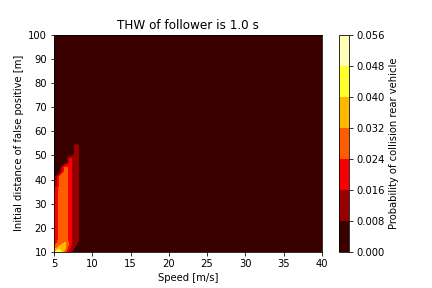
\includegraphics[width=.9\linewidth]{figures/fp_prob_10_100_5_40_10.png}

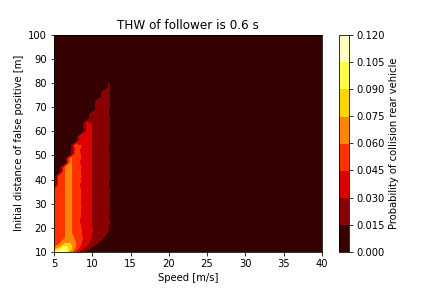
\includegraphics[width=.9\linewidth]{figures/fp_prob_10_100_5_40_06.png}

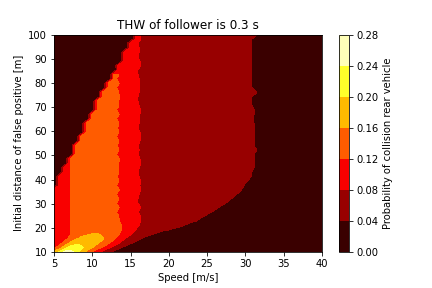
\includegraphics[width=.9\linewidth]{figures/fp_prob_10_100_5_40_03.png}

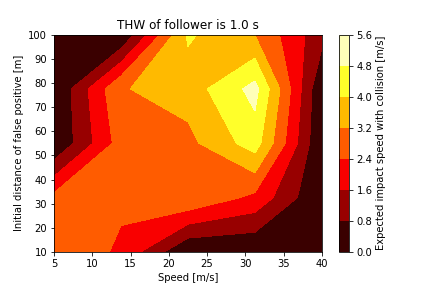
\includegraphics[width=.9\linewidth]{figures/fp_vimpact_10_100_5_40_10.png}

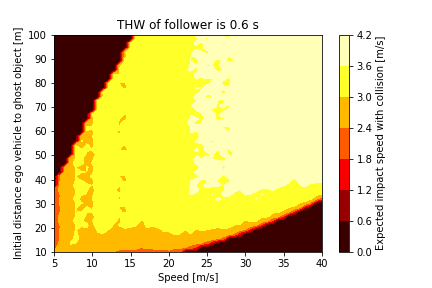
\includegraphics[width=.9\linewidth]{figures/fp_vimpact_10_100_5_40_06.png}

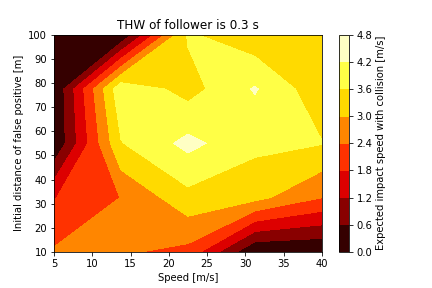
\includegraphics[width=.9\linewidth]{figures/fp_vimpact_10_100_5_40_03.png}



\subsection{Risk of false positives}
\label{sec:results false positives}

\todo{Heatmap with two variables: ego vehicle speed (5 - 40), target speed (0 - 5).}



\subsection{Risk of low-$\mu$ road surface}
\label{sec:results low mu}



\subsection{Risk of graded road}
\label{sec:results slope}
